%!TEX root = ../09-Photoelectric-Effect.tex
\chapter{Photoelectric Effect}


\section{Terminal Voltage}\label{sec:term_volt}%3.1

\textbf{Setup}\\
\begin{figure}[tbp]
	\centering
	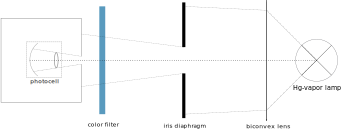
\includegraphics[width=.6\textwidth]{./img/3-1-setup.pdf}
	\caption[Setup for measuring terminal voltage]{\textbf{Setup for measuring terminal voltage} The usage of a Hg-vapor lamp is necessary for sufficiently high photovoltages and -currents, as photons from the Hg-vapor lamp have higher energies than ambient photons.}
	\label{fig:term_volt}
\end{figure}
The setup in \autoref{fig:term_volt} is used to measure the terminal voltage of the photoelectric cell for different wavelengths.
Wavelengths are selected by placing different color filters in the beam path.
The used buffer amplifier is zeroed to allow for high precision measurements.
Varying $\lambda$, the voltage $U$ across the photoelectric cell is measured.

Conservation of energy yields
\begin{align}
	eU &= h\nu+E_\text{A} \nonumber \\
	\Leftrightarrow U &= \frac{hc}{e}\cdot\lambda^{-1}+\frac{E_\text{A}}{e}, \label{eq:energy_balance}
\end{align}
where $E_\text{A}$ denotes the workfunction of the photocathode material.
This equation can be used to compute the ratio $\frac{h}{e}$.

\textbf{Evaluation}\\
\begin{figure}[tbp]
	\centering
	\includegraphics[width=.6\textwidth]{./data/plots/3-1.pdf}
	\caption[Linear regression of terminal voltage over wavelength]{\textbf{Linear regression of terminal voltage over wavelength} Three series of data points are measured and a linear fit for all data sets is applied, as the data was sufficiently reproducible. $a=\SI{922.7}{\volt\nm}$, $b=\SI{-985.3}{\milli\V}$, $R^2=99.5\%$}
	\label{fig:linreg_term_volt}
\end{figure}

A linear fit for the measured data can be seen in \autoref{fig:linreg_term_volt}.
Using \autoref{eq:energy_balance}, the parameters $a$ and $b$ can be identified with $\frac{hc}{e}$ and $\frac{E_\text{A}}{e}$ respectively, yielding
\begin{align*}
	\frac{h}{e} &= \frac{a}{c} \\
	&=\SI{3.08e-15}{\volt\second}
\end{align*}
and
\begin{align*}
	E_\text{A} &= b\cdot e \\
	&=\SI{-985.3}{\milli\eV}.
\end{align*}
The experimentally determined ratio $\frac{h}{e}$ deviates by \num{25.5}\% from the literature value\footnote{\url{www.wolframalpha.com/input/?i=planck+constant+per+elementary+charge}}.
As specified in the lab description, the used photocathode's suface is made of potassium, which has a workfunction\footnote{\url{www.wolframalpha.com/input/?i=workfunction+of+potassium}} of \SI{2.29}{\eV}.
Considering this literature value, the experimentally determined workfunction deviates by \num{56}\%.
It is worth to note that this reproduces data found by other experimenters\footnote{\url{www-ekp.physik.uni-karlsruhe.de/~simonis/praktikum/musterprotokolle/P2/Photoeffekt/Photoeffekt-2013-MatthiasLinster+DominicScheider.pdf}}, which increases the significance of results found in this experiment.
A probable cause of systematic errors influencing the value of the workfunction is the color filters' wavelength specifications as well as their transmission characteristics, which may vary.

\section{Stopping Voltage - Voltage Zeroing}%3.2
\begin{figure}[tbp]
	\centering
	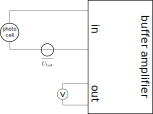
\includegraphics[width=.4\textwidth]{img/3-2-setup.pdf}
	\caption[Setup for measuring stopping voltage]{\textbf{Setup for measuring stopping voltage} $U_\text{bat}$ is tuned to zero the photovoltage.}
	\label{fig:comp_volt}
\end{figure}
\begin{figure}[tbp]
	\centering
	\includegraphics[width=.6\textwidth]{./data/plots/3-2.pdf}
	\caption[Linear regression of stopping voltage over wavelength]{\textbf{Linear regression of stopping voltage over wavelength} A linear fit is applied. $a=\SI{903.1}{\volt\nm}$, $b=\SI{-954.2}{\milli\V}$, $R^2=99.5\%$}
	\label{fig:linreg_comp_volt}
\end{figure}
Using the setup shown in \autoref{fig:comp_volt}, the voltage necessary for zeroing the photovoltage is measured in dependence of the light's wavelength.
\autoref{fig:linreg_comp_volt} shows a linear fit for the measured data.
\autoref{eq:energy_balance} can be used to compute the ratio $\frac{h}{e}$ and workfunction $E_\text{A}$ as
\begin{gather*}
	\frac{h}{e}=\SI{3.012e-15}{\volt\second},\quad E_\text{A}=\SI{-954.2}{\milli\eV}.
\end{gather*}
Using the same literature values as in \autoref{sec:term_volt}, the experimental ratio $\frac{h}{e}$ deviates by \num{27.6}\%, whereas the workfunction deviates by \num{57.8}\%, roughly reproducing the results found in \autoref{sec:term_volt}.
Probable systematic error sources are those mentioned in \autoref{sec:term_volt} and the accuracy of the battery voltage.

\section{Photocurrent}\label{sec:photo_current}%3.3 and 3.4

The current flowing through the photoelectric cell is measured while the voltage across its terminals is held at constant levels ranging from \SIrange{-3}{6}{\volt}.
The experiment is repeated with a neutral density filter in front of the mercury lamp.

\textbf{Setup}\\
A schematic of the setup is shown in \autoref{sch:photocurrent}.
A shunt resistor of $R_\text{shunt} = \SI{100}{\mega\ohm}$ is used, the output voltage $U_\text{out}$ is buffered by the electrometer to minimize the additional load.
The voltage $U_\text{g}$ is generated by a potentiometer connected across a \SI{9}{\volt} battery, it is read from a panel meter.

The actual stopping potential is $U_\text{s} = U_\text{g} - U_\text{out}$, the photocurrent is calculated as $I_\text{ph} = \frac{U_\text{out}}{R_\text{shunt}}$.

\textbf{Evaluation}\\
The measured values for the series with and without filter are shown in \autoref{plt:photocurrent}.
All experiments are done with the \SI{400}{\nm} filter.
There is no measurable reverse current, so measurements for $U_\text{g} < \SI{-1.6}{\volt}$ are omitted.

Both curves start around \SI{-1.5}{\volt} looking similar to the characteristic diode curve.
This voltage represents the maximum kinetic energy of the freed electrons which is equal to $E_\text{k, max} = hf - E_\text{A}$, it is not dependent on light intensity.
For higher stopping potentials, the current approaches the saturation current.
In this region, the electric field attracts all freed electrons to the anode, the quantum efficiency (number of electrons over number of photons) approaches the material dependent maximum.

To approximate the saturation current, a logistic curve is fitted to the data as it is the most accurate model tested:
\begin{equation*}
	I_\text{ph}(U_\text{s}) = \frac{I_\text{sat}}{1 + \mathrm{e}^{-b (U_\text{s} - U_0)}},
\end{equation*}
resulting in
\begin{gather*}
	I_\text{sat} = \SI{37}{\nA}, \quad U_0 = \SI{1.64}{\volt}, \quad b = \SI{1.28}{\per\volt} \tag{no filter}\\
	I_\text{sat} = \SI{23}{\nA}, \quad U_0 = \SI{1.86}{\volt}, \quad b = \SI{1.15}{\per\volt}. \tag{filter}\\
\end{gather*}

The saturation current is proportional to the filter's transmittance, so the transmittance can be calculated as
\begin{equation*}
	T = \frac{I_\text{sat, filter}}{I_\text{sat,no filter}} = \num{0.62}.
\end{equation*}

\begin{figure}[tbp]
	\centering
	\includegraphics[width=.4\textwidth]{img/photocurrent.pdf}
	\caption[Setup for measuring Photocurrent]{\textbf{Setup for measuring Photocurrent}, the output voltage is buffered by the amplifier}
	\label{sch:photocurrent}
\end{figure}

\begin{figure}[tbp]
	\centering
	\includegraphics[width=.8\textwidth]{data/plots/photocurrent.pdf}
	\caption[Photocurrent versus Stopping Potential]{\textbf{Photocurrent versus Stopping Potential}, constant wavelength $\lambda = \SI{400}{\nm}$}
	\label{plt:photocurrent}
\end{figure}

\section{Stopping Voltage - Current Zeroing}%3.5
\begin{figure}[tbp]
	\centering
	\includegraphics[width=.6\textwidth]{./data/plots/3-5.pdf}
	\caption[Linear regression of stopping voltage over wavelength]{\textbf{Linear regression of stopping voltage over wavelength} A linear fit is applied. $a=\SI{1142.8}{\volt\nm}$, $b=\SI{-1.51}{\V}$, $R^2=98.3\%$}
	\label{fig:linreg_comp_curr}
\end{figure}
The same setup as in \autoref{sec:photo_current} is used, this time zeroing the photocurrent by tuning the battery voltage.
One data set for varying wavelengths is recorded and a linear fit as in \autoref{sec:term_volt} is applied.
\autoref{fig:linreg_comp_curr} shows the fit of this linear model, yielding
\begin{gather*}
	\frac{h}{e}=\SI{3.81e-15}{\volt\second},\quad E_\text{A}=\SI{-1.51}{\eV}.
\end{gather*}
Using the same literature values as in \autoref{sec:term_volt}, the experimental ratio $\frac{h}{e}$ deviates by \num{8.5}\%, whereas the workfunction deviates by \num{33.2}\%.
These results are much closer to the literature values than those found in \autoref{sec:term_volt}.
